\subsection{Kantdetektion}

Vi kan bruge første- og andenordens differentialer til at finde ændringer i intensitet, med det formål at finde kanter. Se Figur~\ref{fig:differential-edge-detection}. 

\begin{figure}[H]
	\centering
	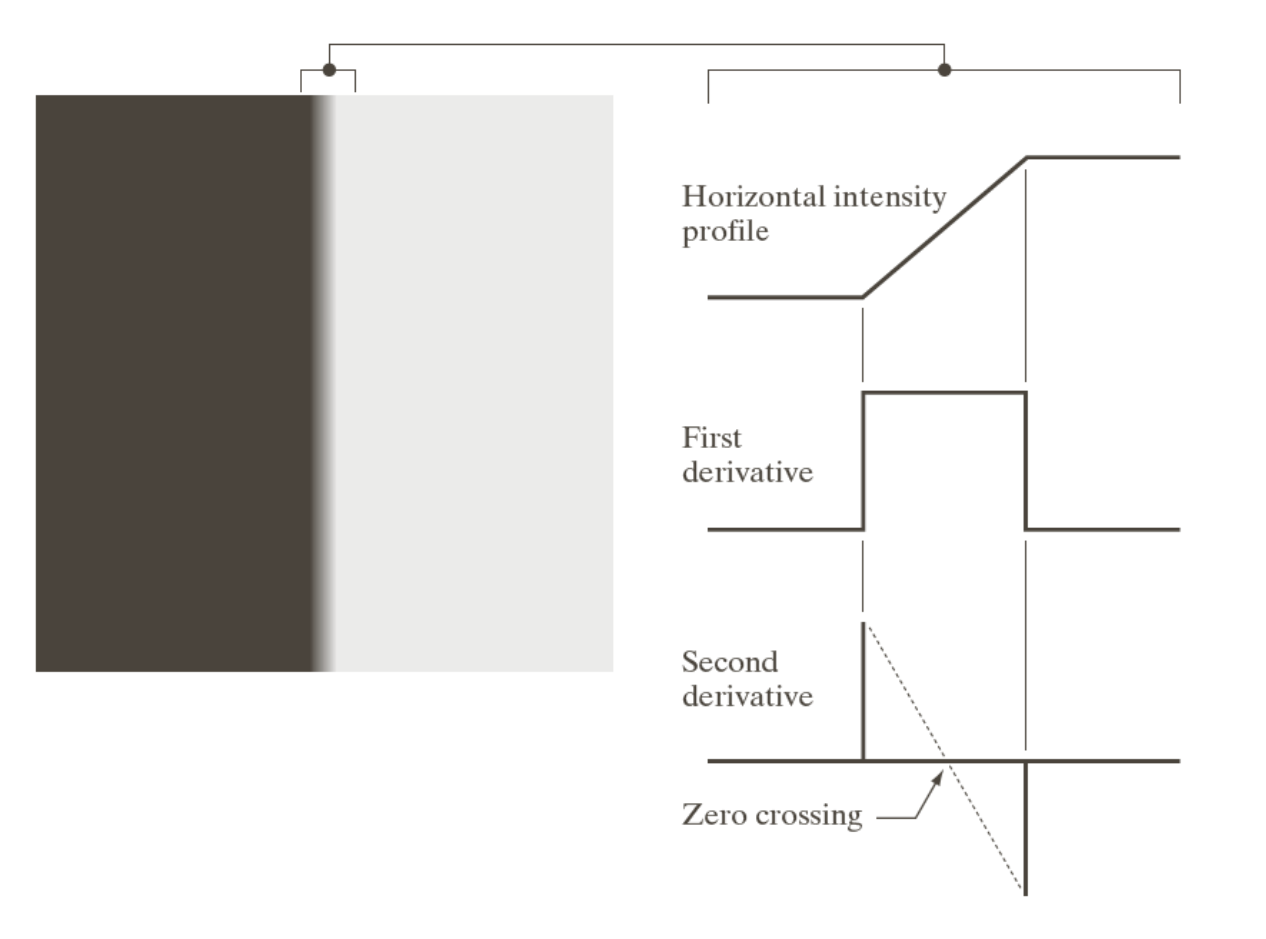
\includegraphics[width=0.75\linewidth]{figs/spm03/differential-edge-detection}
	\caption{Hvordan først- og andenordens differentialer kan bruges til at finde kanter.}
	\label{fig:differential-edge-detection}
\end{figure}

Til at finde kanter med simple spatiale filtre kan vi eksempel vis bruge Prewitt eller Sobel, se Figur~\ref{fig:gradient-filters} til at finde store intensitetsforskelle i billedet.

\begin{figure}[H]
	\centering
	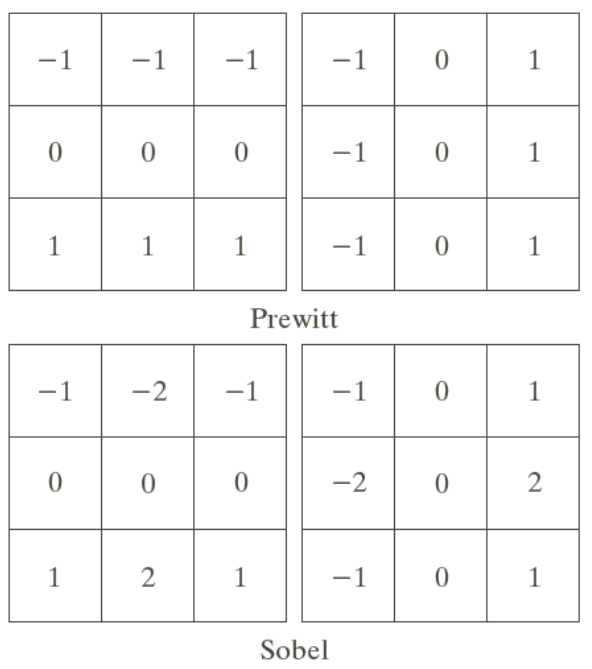
\includegraphics[width=0.5\linewidth]{figs/spm03/gradient-filters}
	\caption{Prewitt og Sobel filtre.}
	\label{fig:gradient-filters}
\end{figure}

Disse filtre kan selvfølgelig også bruges til at finde diagonale kanter, de skal bare drejes, se Figur~\ref{fig:prewitt-and-sobel-diag-filter}.

\begin{figure}[H]
	\centering
	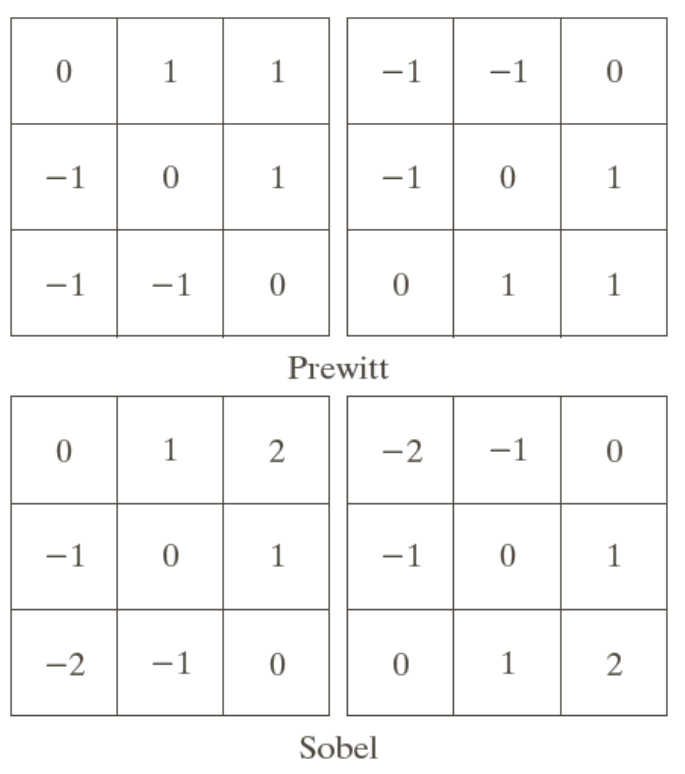
\includegraphics[width=0.5\linewidth]{figs/spm03/prewitt-and-sobel-diag-filter}
	\caption{Diagonale Prewitt og Sobel filtre.}
	\label{fig:prewitt-and-sobel-diag-filter}
\end{figure}
